\section{Basic structure of an Android App}
Android is an open source operating system for mobile phones and tables based on the Linus kernel (\cite{androiddef}). Android apps are distributed on Google Play, a service owned by Google. To build and Android app Google offers the Android \gls{SDK}, containing sample projects, necessary Android libraries and an Android emulator. Additionally, Google recommends to use the official Android \gls{IDE} Android Studio, which is based on IntelliJ IDEA and offers many useful tools, including testing frameworks, a \gls{GUI} for screen layouts, and the build tool Gradle (\cite{androidstudio}). The concepts and Android components discussed throughout this chapter are taken from the Android Developer reference (\cite{androidreference}), training (\cite{androidtraining}), and \gls{API} guides(\cite{androidguides}) found online.

An Android app consists of  at least one activity which can contain one or more fragments --- both activities and fragments are basic Android application components. An activity, in the Android context, is a Java class that extends the Activity class. It manages a screen and is needed to display any user interface. Fragments implement a specific user interface or behaviour and should, ideally, be modular so they can be reused with multiple activities and in different screen configurations. Both components have their own lifecycles and events during the apps runtime. Activities feature methods such as onCreate(), onStart(), onStop(), and onFinish(), which can be overwritten to implement logic that is executed at different points in it’s life. Same applies for a fragment, but where an activity can stand alone, a fragment always needs to be attached to an activity; it is connected to that activity's lifecycle --- is the activity stopped, the fragment will stop as well.
When containing fragments, the activity’s job is that of managing those fragments through getters and setters and orchestrating the communication between fragments, which is done with callbacks defined in the fragments.

Activities and Fragments can house ViewGroups and Views, which define different UI components for Android. Such a view would be a TextView, which displays one multiple lines of text. Viewgroups and views can be extended in custom classes to implement non-standard behaviour.

\section{Basic Components of an Android App}

\subsection{Activity}
The Activity class is needed to display any user interface and as such usually has a single purpose --- handling a login would be such a purpose. An app consists of one or more activities that are in some way connected to each other (\cite{activities_in_app}). An activity can embed multiple fragments --- those fragments then live in a ViewGroup inside the activity's own view hierarchy (\cite{androidfragment}).  

\subsection{Actionbar}
The actionbar located at the top of an app and has several important functions. It displays the application name or the title of an activity, houses the action buttons, and the action overflow. Action buttons should contain the most commonly and important actions used in an app (\cite{actionbar}). The action overflow contains action buttons that are hidden from plain view, either because the actionbar was not wide enough to show all buttons or because of a deliberate design decision. Such a decision is usually made when the button in question is connected to an action that is rarely used, e.g. renaming something, or when the action has far-reaching consequences and shouldn't be near buttons that are used frequently, lest the user accidently hits it. Such an action could be the deletion of the currently edited pattern, in case of an knitting app. 

\subsection{Fragment}
The Fragment class ususally implements a specific user interface or behaviour and should, ideally, be modular, so that they can be reused within multiple activities or in different screen configurations. Just like an activity a fragment has its own lifecycle, see \reffigure{fig:fragment_lifecycle}.

\begin{wrapfigure}{O}{0.33\textwidth}
    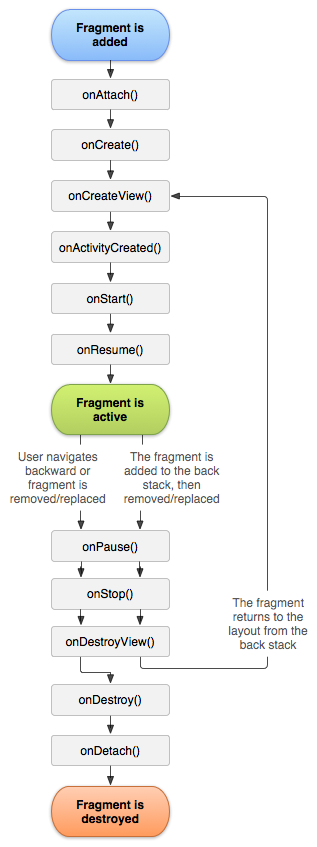
\includegraphics[width=1.0\linewidth]{images/fragment_lifecycle.png}
   	\caption[The lifecycle of a fragment. \protect\newline{\small at: \url{https://developer.android.com/images/fragment_lifecycle.png} (last accessed: 2016-08-09)}]{The Fragment life cycle}
   	\label{fig:fragment_lifecycle}
\end{wrapfigure}

A fragment's creation is always embedded in an activity (\cite{androidfragment}) --- forcing the fragment to pause or stop alongside its parent activity's lifecycle. Fragments can also house viewgroups and views and are intented to function as interchangeable modules, e.g. as \gls{UI} modules for an app that runs on devices of varying sizes and that wants to present the user with a dynamic \gls{UI} fit to suit the screen size (see \reffigure{fig:fragments_uimodules}).

\begin{wrapfigure}{O}{0.5\textwidth}
    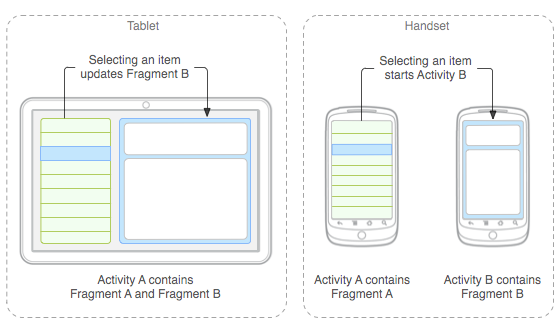
\includegraphics[width=1.0\linewidth]{images/fragments.png}
   	\caption[Two fragments of one activity and their layout on two different screen sizes. \protect\newline{\small at: \url{https://developer.android.com/images/fundamentals/fragments.png} (last accessed: 2016-08-09)}]{Two fragments of one activity and their layout on two different screen sizes} 
   	\label{fig:fragments_uimodules} 
\end{wrapfigure}

Android offers different fragment subclassse with predefined behavior, such as the DialogFragment class, that opens a fragment as a floating dialog by default (see \reffigure{fig:dialog_fragment}). \todo{add figure dialog fragment} Communication between different fragments needs to be handled by the activity, which manages the fragments. An activity communicates with a fragment by keeping a reference to the fragment and calling its public methods. On the other hand the fragment should not possess a reference to its parent activity --- instead the parent activity should implement a callback interface defined inside the fragment (\cite{fragment_event_callback}). A good practive to enforce the implementation of a fragments callback interface is to check for its existence when the fragment is attached to the activity --- example code proposed by the Android Developer guide concerning how to check for this can be seen in \reflisting{lst:callback_interface} (\cite{fragment_event_callback}).

\begin{lstlisting}[language=JAVA, caption=Example code for enforcing the implementation of a callback interface, label=lst:callback_interface]
public static class FragmentA extends ListFragment {
    OnArticleSelectedListener mListener;
    ...
    @Override
    public void onAttach(Activity activity) {
        super.onAttach(activity);
        try {
            mListener = (OnArticleSelectedListener) activity;
        } catch (ClassCastException e) {
            throw new ClassCastException(activity.toString() + " must implement OnArticleSelectedListener");
        }
    }
    ...
}
\end{lstlisting}

\subsection{View}
Views are the most basic block that the \gls{UI} is built from (\cite{android_view}). A view's bounds are always rectangular and its position is defined by its top and left coordinates with the point of origin at the top left. It is the view's job to handle its drawing and event handling. For this the view has the predefined methods onDraw() and onTouchEvent(), respectively. The view class is also the base for viewgroups which in turn are the base for layouts, containers for other views or viewgroups.
The views from a window are arranged in a tree structure. Views can be added to this tree statically, by specifying them in an \gls{XML} layout file, or dynamically, from code. Android comes with plenty of view subclasses, specialized in acting as controls or displaying specific types of content, e.g. text or images. If the pre-existing views don't match a developer's needs, they can also implement a custom view to take control of the drawing and the event handling as it fits their requirements. For this the onDraw() method can be overridden and custom operations can then be executed on the Canvas object that is contained in the method parameters.

Android ships with many subclasses of View, specialized for displaying text (TextView), or a button (Button). The view class is also the basis for ViewGroups, to which the layouts, e.g. LinearLayout and RelativeLayout, belong to. Views in a window are bundled together as a tree with a layout being the top-most root. To add views to an activity or fragment the views can be declared in the corresponding \gls{XML} layout or from code. 

\subsection{Storage}
\label{android_storage}
File storage in Android devices is separated into ``internal'' and ``external'' storage --- this refers to the fact, that Android devices often times have a built-in, non-removable memory and an external, removable medium in the form of an SD or a micro SD card (\cite{android_storage}). This storage separation even exists on devices with only built-in memory --- in such cases the storage is partitioned into ``internal'' and ``external'' partitions. This assures that the concept of two storages persists across all devices and \gls{API} levels. The internal storage is inaccessible by the user under normal circumstances --- exception to that is when the user has root privileges, e.g. on a rooted phone. This storage houses, among other things, files from apps, e.g. databases. These files are only accessible by the app that originially places them in the interal storage --- neither user nor other apps can access them. Files are removed when the app they belong to is uninstalled. 
The external storage on the other hand is more public. Files placed here can be read and written by user and other apps and they even remain after the app they orignated from is uninstalled. When working with the external storage it is important to check that it is not currently used as \gls{USB} storage by a computer the device is connected to.
Apps have by default read and write access to the directory they are installed in on the internal storage, but to access the external storage the app requires that the user grants the app a specific permission. This permission needs to be declared in the app's manifest file, a XML file that every app must have. This file contains information required by the Android system to allow the app to run, such as the activities contained in the app and the permissions the app requires. Beginning in Android 6.0 (\gls{API} level 23) apps targeting that Andoir version need to request and aquire dangerous permissions at run time (\cite{android_permissions}), whereas before the app was given all permissions listed in its manifest upon agreeing to a dialog popup when installing the app. Dangerous permissions cover access to the user's private data or to affect areas where the user stores their data or data that other belong to other apps (\cite{android_permissions}). Since the user can revoke permissions for apps at any given time the developer needs to take measures to keep the app running even when some features need to be disabled because of missing permissions.  
